% !Mode:: "TeX:UTF-8:Hard"
\ifx \allfiles \undefined
\documentclass[a4paper,12pt,twoside]{book}
\usepackage{CJKutf8}
\usepackage[T1]{fontenc}
\usepackage{pifont}
\usepackage{graphicx}
\usepackage{capt-of}
\usepackage{color}
\newcommand{\linuxcommand}[1]{\texttt{\textcolor{blue}{\$ #1 \Pisymbol{psy}{191}}}}
\newcommand{\op}[1]{\textcolor{blue}{-#1}}
\newcommand{\hotkey}[1]{\framebox{#1}}
\newenvironment{screen}{\sffamily}{\rmfamily}

\begin{document}
\begin{CJK*}{UTF8}{song}
\title{基础知识}
\author{赵岩}
\date{}\maketitle

\else
\chapter{Basic Knowledge}
\fi

\section{General Knowledge}

	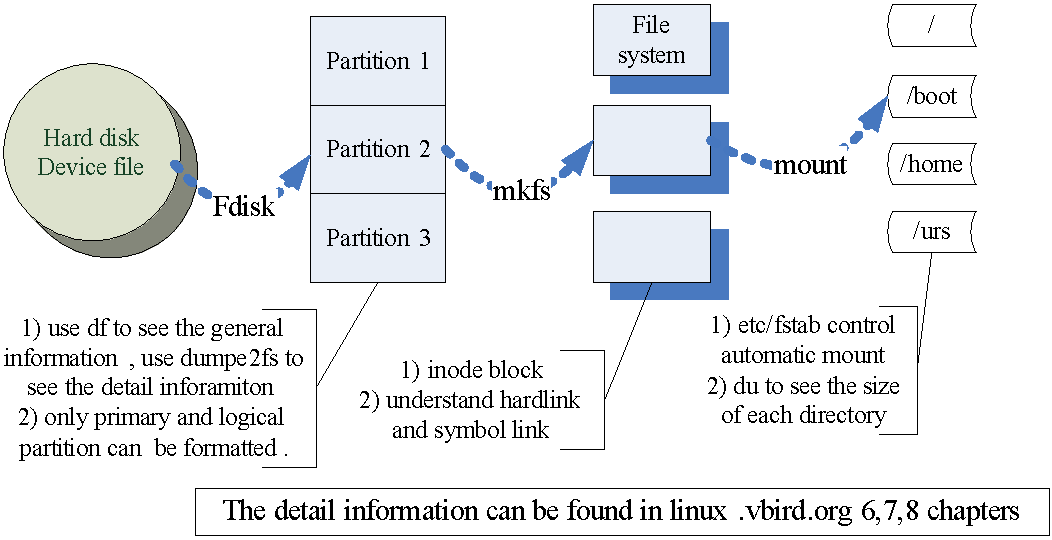
\includegraphics[scale=0.8]{pics/basic_file_system_clip}	
	\begin{itemize}
	\item You can google "where is my IP address'' to get you external IP, or use \linuxcommand{ipconfig} to know your internal IP. \linuxcommand{host} can know IP or host name from each other. Another Interesting tool is \linuxcommand{netstat} can tell you what connections are there in your computer. and \linuxcommand{traceroute} can trace the path in connection. They are some useful Internet connection tool.
	\item There are two kinds of clips, one is local clip, you only can switch data within this application, such as use Ctrl+C in kile, you only can paste in kile
	if you want to paste sth to other application, you should use shift+mouse selection and copy to xclip. middle button can paset it. In Emacs, Alt+W will copy content to global clip.
	\item *.so is shared dynamic library in linux
	\item Don't log in root, you can use \linuxcommand{sudo } follow your command
	\item Ctrl+Alt+F1\ldots F6 switch terminal. Ctrl+Alt+F7 return back to GUI
	\item install some perl programe, If you want to install in your own directory, you can add PREFIX. That will assure you have permission on it \\
  	 perl Makefile.PL  
    \begin{verbatim}
    perl Makefile.PL PREFIX=\storage\yzhao
    make
    make test
    make install
    \end{verbatim}
	\item Under linux, if you want to install programme. If there are source\_code. \\
    \begin{verbatim}
	./configure 
	make
	make install
    \end{verbatim}
	you should download from internet directly, you can't unzip it in windows. You should use tar command to unzip under linux. If you don't have root account, you can ./configure --prefix=~/program. it will compile source first, when you make install. It will copy some files to ~/program/bin or ~/program/share.
	./Configure use Makefile.in to produce Makefile. They are a set of automatic tools. You can see them in c++ web directory, but they are a little complicated, Kdevelop also use them. Just know them. OK!
	\item to make less show Chinese, \linuxcommand{export LESS=-isMrf} I don't know what it means?
	\item \linuxcommand{nice commandname \&} means that you run command friendly with other(not occupy all resources) and run it at background. Skuld may be a UNIX server!
	\item usually, virtual box think right Ctrl as default host key, it's not convinent in linux, because most of move command need right Ctrl, so you need change it.
	In window, run VBoxManage.exe setextradata global GUI/Input/HostKey 165 can change it to right Alt. Here, I need to explian, the 165, it's virtual keycode defined by
	microsoft. you can find detail in google. Now I change it to Win\_L, value is 91.
	\item There are AltGr key to input multi-language character, but I don't need it by now, according to my laptop layout, I need to change it to Alt, so I
	can use move command shortcut. and define win\_menu to Ctrl. I finish it as follow: \\
	1) use \linuxcommand{xev} get keycode, AltGr is 108 and win\_menu is 135 \\
	2) create your own .Xmodmap and write keycode 108 = Alt\_L\\
	3) in .bashrc, add some statements\\
	xmodmap -e "add Contrlo = Menu'' (this statement is very important)\\
	xmodmap -e "keycode 133 = Control\_R''\\
	\item  about keyboard shortcut, I have good idea, that is to use left Ctrl and Alt together, because you can use your thumb to press Alt and use palm to
	press Ctrl\_L,(Even in my three laptops, I also can press Ctrl\_L easily by palm).
	So a shortcut can be defined below:
	\[ \left\{ \begin{array}{cl}
	            \textrm{move} & \left\{ \begin{array}{c} \textrm{other: Ctrl\_L} \\ \textrm{emacs: Alt\_L} \end{array}  \right. \\
		    \textrm{select} & \left\{ \begin{array}{c} \textrm{other: Ctrl\_L+Shift\_L} \\ \textrm{emacs: Alt\_L+Shift\_L} \end{array}  \right. \\
	           \end{array} \right. + \left\{ \begin{array}{c}
						\textrm{left character: J} \\
						\textrm{right character: L}\\
						\textrm{upward: I}\\
						\textrm{downward: k}\\
						\textrm{left word: U}\\
						\textrm{right word: O} \\
						\textrm{begin line: H}\\
						\textrm{end line: ;}\\
						\end{array} \right.
	\]
	Delete command is below: \\
	\[ \textrm{delete} \left\{ \begin{array}{l}
	            \textrm{left character: Backspace}  \\
		    \textrm{right charcter: Ctrl\_L+N} \\
		     \textrm{left word: Ctrl\_L+Backspace}  \\
		    \textrm{right word: Ctrl\_L+M} \\
		     \textrm{line: Ctrl\_L+P}  \\
	           \end{array} \right.
	\]
	
	Question 1: why always left Ctrl? \\
	Answer: Now, if you are smart enough, you can found that there is rules inside. all the commands is left Ctrl add right hand character, becuase left Ctrl can be
	pressed by left palm and right hand is more flexible than left hand when you click the different character. \\
	Question 2: why other use Ctrl and Emacs use Alt. \\
	Answer: In common applications, Alt has been assign to trigger menu item, such as Alt+F will trigger File menu, so, I must use Ctrl. In Emacs, on the contrary,
	Ctrl has been used to trigger some common commands, so I use Alt key( and Alt is used not often as Ctrl).\\
	Question 3: How can I export my custom shortcut to other computers \\
	Answer: There are two kind of shortcut one is kate and other is kile, they store in .kde/share/apps/katepart/katepartui.rc and \linebreak[4] .kde/share/apps/kile/kileui.rc
	you can copy them and cover them in your computer. If version is different, Maybe it's a little difficult. But you can just do it within the application, it
	don't need very long time. \\
	 目前,这些键盘的定义我还没有在实践中使用过。毕竟,用箭头键太直接了,而按住ctrl在一些笔记本上不是太方便。 不过,他们依旧是一个很好的建议,以后当你使用大键盘,或者是比较密集的进行编辑工作的时候,还是非常值得尝试一下的。 
	
	\end{itemize}
\section{Environment variable}
	\begin{itemize}
	\item you should create your own bin folder under your own directory. And save your own script into it.
	Echo \$PATH will show your path setting. You can export PATH=\$PATH:/storage/yzhao/bin (add path in the end.)
	to add a new directory. Linux use : but windows use ; why windows use different?
	\item \linuxcommand{export DEPART=Sale} and \linuxcommand{DEPART=Sale ; export DEPART} they means the same. If the export statement in a script file,
	you must use \linuxcommand{Source a.sh} or \linuxcommand{. a.sh} to run the script file, then It will affect the continuous processing. source only run
	in father bash, it doesn't run in a child shell.
      \item setenv is csh command, in bash, you can use export directly.
	\item env list all the environment variables
	\item EDITOR can specify you default editor in your system.
	\item \linuxcommand{set} list all the local environment variables, that is more than env command. \linuxcommand{unset} to delete an environment variable
	\item getconf can get some system variable, such as
getconf ARG\_MAX, you can use xargs -n 50 to make command
satisfy the ARG\_MAX
	\end{itemize}

\ifx \allfiles \undefined
\end{CJK*}
\end{document}
\fi
